\documentclass[12pt]{article}
\usepackage[czech]{babel}
\usepackage[utf8]{inputenc}
\usepackage[plainpages=false,pdfpagelabels,unicode]{hyperref}
\usepackage[pdftex]{graphicx}
\usepackage[margin=2cm, includefoot]{geometry}

\begin{document}

\title{Určení koncentrace kyslíkových radikálů pomocí aktinometrie.}
\author{Pavel Ondračka a~Vlasta Štěpánová}
\maketitle

\section{Úvod}
Aktinometrie je metoda používaná pro určování koncentrace kyslíkových radikálů. Tato metoda se využívá při plazmovém leptání a~plazmochemických depozicích oxidových vrstev. Principem metody je porovnání intenzity emisní čáry radikálu (kyslíku) a~aktinometru, což je inertní plyn, který se v~malém množství přidává do plazmatu (v našem případě argon).

\section{Teorie}
Při našem měření v~kyslíkovém výboji jsme se rozhodli pozorovat emisní čáru kyslíku ($2s^22p^3(^4S^*)3s$ $^3S^*$ -- $2s^22p^3(^4S^*)3p$ $^3P$) na vlnové délce 844.625\,nm a~emisní čáru argonu ($3s^23p^5(^2P^*_{3/2})4s$ $^2[3/2]^*$ -- $3s^23p^5(^2P^*_{3/2})4p$ $^2[3/2]$) na vlnové délce 763.51\,nm. K excitaci kyslíkových radikálů dochází buďto excitací atomu kyslíku srážkou s~elektronem nebo disociativní excitací elektronem ze základní hladiny molekuly. Zhášení tohoto excitovaného stavu kyslíku můžeme zanedbat vzhledem k jeho velmi krátké době života a~nízkému tlaku. 

Předpokládáme, že excitované stavy $X_i$, obsazované zejména nepružnou srážkou elektronu s~atomem v~základním stavu $X$, následně deexcitují přechodem ze stavu $X_i$ na stav $X_j$ vyzářením fotonu $h\nu_{ij}$.

Intenzitu emisní čáry $I_{ij}$ atomu $X$ můžeme potom zapsat jako:
%
\begin{equation}
I_{ij}^X = C (\lambda_X) \frac{h \nu_{ij} A_{ij} n_\mathrm{e} k_\mathrm{e}^{X_i} } { ( \sum{A_{ij} + [Q] k_{Q}} )} [X] \,\, \mathrm{,} \label{i1}
\end{equation}
%
kde $C (\lambda_X)$ je konstanta úměrná spektrální citlivosti měřícího přístroje, $\nu_{ij}$ je frekvence emitovaného fotonu, $A_{ij}$ je Einsteinův koeficient přechodu $(i \rightarrow j)$, $n_\mathrm{e}$ je koncentrace elektronů, $k$ jsou rychlostní konstanty příslušných procesů, $\sum{A_{ij}}$ je suma všech radiativních přechodů, $[Q]$ je koncentrace částic $Q$ a~$[X]$ je koncentrace atomů $X$. 

Rychlostí konstanty můžeme vypočítat ze vztahu
%
\begin{equation}
k_\mathrm{e}^{X_i} =  \sqrt{\frac{2}{m}} \int_0^\infty \sigma_\mathrm{e}^{X_i}(E)\,\sqrt{E}\,f(E)\,\mathrm{d}E \, \mathrm{,} \label{vzoreck}
\end{equation}
%
kde $E$ je energie elektronů, $\sigma_\mathrm{e}^{X_i}(E)$ je účinný průřez příslušného procesu částice $X$ a~$f(E)$ je rozdělovací funkce energie elektronů. 

V našem případě se jedná o~Maxwellovo rozdělení, které je definováno takto:
%
\begin{equation}
f(E) = \frac{4\pi}{m} \sqrt{\frac{2}{m}} \left( \frac{m}{2 \pi k T} \right)^{3/2} \sqrt{E} \,\,\mathrm{e}^{\frac{-E}{kT}} \, \mathrm{,} 
\end{equation}
%
kde kde $m$ je hmotnost elektronu, $k$ je Boltzmannova konstanta a~$T$ je teplota elektronů.

Ze vztahu (\ref{i1}) dostáváme vztah pro poměr intenzit emisní čáry atomu $X$ z~hladiny 1 a~emisní čáry atomu  $Y$ z~hladiny 2:
%
\begin{equation}
\frac{I_1^X}{I_2^Y} = 
\frac{C (\lambda_{X_1})}{C (\lambda_{Y_2}) }
\frac{h \nu_1 A_1^X } {h \nu_2 A_2^Y} 
\frac{k_\mathrm{e}^{X_1} }{k_\mathrm{e}^{Y_2} }  
\frac{ ( \sum{A_{i}^Y + [Q] k_Q^Y} ) }{ ( \sum{A_{i}^X + [Q] k_Q^X} ) }
\frac{[X]}{[Y]}
 \,\, \mathrm{,} \label{i2}
\end{equation}
%
ze kterého plyne, že můžeme vypočítat koncentraci druhého druhu atomů z~poměru intenzit emisních čar, pokud známe koncentraci prvního druhu atomů a~potřebné konstanty. 

Nyní vztah (\ref{i2}) již pro konkrétní plyny (argon a~kyslík):
%
\begin{equation}
\frac{I_{844}^\mathrm{O} } {I_{750}^\mathrm{Ar}} =
\frac{C (844\,\mathrm{nm})} {C (740\,\mathrm{nm}) }
\frac{750} {840} 
\frac{ A_{844}^\mathrm{O} } { A_{750}^\mathrm{Ar} }
\frac{ k_\mathrm{e}^\mathrm{3P} [\mathrm{O}] + k_\mathrm{de}^\mathrm{3P} [\mathrm{O}_2] } {k_\mathrm{e}^\mathrm{2P_1} [\mathrm{Ar}]}  
\frac{\sum_j{A_{ij}^\mathrm{Ar}}  } { \sum_j{A_{ij}^\mathrm{O}} }
\,\, \mathrm{.} \label{i3}
\end{equation}
%
Čáru argonu jsme zvolili úmyslně poblíž kyslíkové čáry, abychom tak minimalizovali korekci na citlivost přístroje. Vztah (\ref{i3}) se od vztahu (\ref{i2}) liší přítomností disociativní excitace molekuly kyslíku O$_2$.

Zavedením stupně disociace
%
\begin{equation}
\alpha_\mathrm{d} = \frac{[\mathrm{O}]_\mathrm{pl}}{2[\mathrm{O}_2]_\mathrm{dod}}
\end{equation}
%
a využitím zákona zachování hmoty částic dodávaných do plazmatu a~vzniklých v~plazmatu
%
\begin{equation}
\eta = \left( \frac{[\mathrm{O}_2]}{[\mathrm{Ar}]} \right)_\mathrm{dod}
 = \left( \frac{2[\mathrm{O}_2] + [\mathrm{O}]}{2[\mathrm{Ar}]} \right)_\mathrm{pl}
\end{equation}
%
dostáváme tzv. aktinometrický signál
%
\begin{equation}
\frac{1}{\eta C}
\frac{I_{844}^\mathrm{O}}{I_{750}^\mathrm{Ar}} = 
\frac{k_\mathrm{de}^\mathrm{3P}}{k_\mathrm{e}^\mathrm{2P_1}} + 
\alpha_\mathrm{d}
\left(
2\frac{k_\mathrm{e}^\mathrm{3P}}{k_\mathrm{e}^\mathrm{2P_1}} - 
\frac{k_\mathrm{de}^\mathrm{3P}}{k_\mathrm{e}^\mathrm{2P_1}}
\right) \, \mathrm{,}
\end{equation}
%
kde konstanta $C$ zastupuje všechny konstanty včetně Einsteinových koeficientů a~přístrojové funkce.

Podmínky pro určení stupně ionizace
%
\begin{equation}
\frac{1}{\eta C}
\frac{I_{844}^\mathrm{O}}{I_{750}^\mathrm{Ar}} < 2k_\mathrm{e} 
 \,\,\,\,\,\,\,\, \mathrm{pro} \,\, \alpha_\mathrm{d}=1 \,\mathrm{,}
\label{podm1}
\end{equation}
%
%
\begin{equation}
\frac{1}{\eta C}
\frac{I_{844}^\mathrm{O}}{I_{750}^\mathrm{Ar}} > k_\mathrm{d} 
 \,\,\,\,\,\,\,\, \mathrm{pro} \,\, \alpha_\mathrm{d}=0 \,\mathrm{,}
\label{podm2}
\end{equation}
%
kde $k_\mathrm{d} = k_\mathrm{de}^\mathrm{3P}/k_\mathrm{e}^\mathrm{2P_1}$, $k_\mathrm{e} = k_\mathrm{e}^\mathrm{3P}/k_\mathrm{e}^\mathrm{2P_1}$ v~praxi se může někdy stát, že tato podmínka splněna není z~důvodů nečistoty v~aparatuře nebo projevu vakuové netěsnosti.

Když známe koncentraci dodávaného molekulárního kyslíku, tak můžeme nyní určit absolutní koncentraci atomárního kyslíku vzniklého ve výboji jako
%
\begin{equation}
[\mathrm{O}] = 2 \alpha_\mathrm{d}[\mathrm{O}_2]_\mathrm{dod} \,\mathrm{.}
\end{equation}
%



\section{Měření}

\subsection{Experimentální uspořádání}
Úloha byla realizována na reaktoru zvaném ,,Temelín''. Jedná se o~reaktor kulovitého tvaru z~nerezové oceli o~vnitřním průměru 500\,mm. Uvnitř reaktoru jsou dvě diskové elektrody o~průměrech 80\,mm. Horní buzená elektroda je obklopena uzemněným stínícím prstencem bránícím rozšiřování výboje nad elektrodu.  Dolní elektroda je uzemněna. Mezi elektrodami hoří vysokofrekvenční výboj o~frekvenci 13,56\,MHz. Tlak v~reaktoru se měří pomocí dvou manometrů o~různém rozsahu:

\begin{itemize}
\item kapacitron		(Leybold-Heraus DM21) 		rozsah 0,01--133\,Pa
\item baratron 		(MKS Instruments PR4000)		rozsah 0,001--6\,Pa
\end{itemize}

Čerpací systém aparatury tvoří turbomolekulární vývěva, membránová vývěva a~ventily. Turbomolekární vývěva od firmy Pfeiffer-Vacuum (typ TPH 450H) má čerpací rychlost 450\,l/s. Membránová vývěva od téže firmy slouží k předčerpání turbomolekulární vývěvy a~má minimální čerpací rychlost 1,8\,m$^3$/h. Čerpání je připojeno k dolní části reaktoru, pod spodní elektrodou. Systém vývěr oddělují od reaktoru ventily, které umožňují omezení čerpací rychlosti. Právě přes lamelový ventil byla aparatura čerpána i v~našem případě, takže čerpací rychlost byla omezena. 

Plyny jsou do reaktoru připouštěny přes vnitřní trubici v~horní elektrodě. Průtok plynů je potřeba regulovat citlivě, aby se do reaktoru připustilo jen velmi malé množství a~aktinometr tak nenarušil původní strukturu plazmatu. Pro nastavení průtoku plynu byly použity dva průtokoměry Bronkhorst.

Měření bylo provedeno na optickém emisním spektrometru Avantes (Avaspec - 2040TBC-2). Spektra byla analyzována pomocí programu Spectrum Analyzer. Korekci intenzity jsme provedli podělením našeho spektra citlivostní křivkou (obrázek \ref{citlivost}). Korekce pro náš spektrometr bohužel nebyla přímo dostupná v~programu Spectrum Analyzer.

\begin{figure}[htbp]
\begin{center}
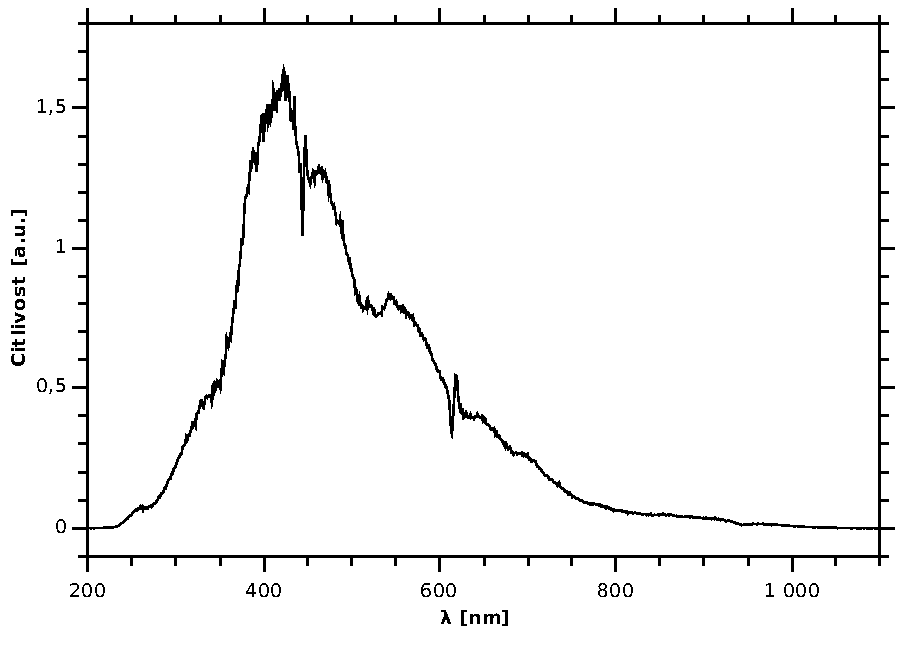
\includegraphics[width=13cm]{citlivost.pdf}
\caption{Citlivost spektrometru Avaspec.}
\label{citlivost}
\end{center}
\end{figure}

\subsection{Rychlostní a~Einsteinovy koeficienty}
Einsteinovy koeficienty byly zjištěny z~databáze NIST:
$$ A_{763,51}^\mathrm{Ar} = 2,45 \cdot 10^7\,\mathrm{s}^{-1} $$
$$ A_{844,625}^\mathrm{O} = 3,22 \cdot 10^7\,\mathrm{s}^{-1} $$
$$ \sum_j A_{ij}^\mathrm{O} = 9,66 \cdot 10^7\,\mathrm{s}^{-1} $$
$$ \sum_j A_{ij}^\mathrm{Ar} = 6,81 \cdot 10^7\,\mathrm{s}^{-1} $$

Rychlostní koeficienty byly spočítány pro teplotu 3\,eV ze vztahu (\ref{vzoreck}), účinné průřezy byly použity ze zadání. Teplota 3\,eV byla zvolena jako typická teplota a~protože dřívější měření teploty v~reaktoru pomocí Langmuirovy sondy nedávalo uspokojivé výsledky. Je nutno podotknout, že tento přístup má neblahý vliv na přesnost měření, jednak proto, že skutečná teplota mohla být výrazně odlišná, a~navíc proto, že skutečná teplota (a s~ní i rychlostní koeficienty) se pravděpodobně v~průběhu měření měnily v~závislosti na podmínkách v~reaktoru (výkon, tlak), což není v~následujících výpočtech nijak zohledněno. 
$$ k_\mathrm{e}^\mathrm{Ar} = 3,37 \cdot 10^{-11}\,\mathrm{cm}^3\,\mathrm{s}^{-1} $$
$$ k_\mathrm{e}^\mathrm{O} = 6,75 \cdot 10^{-11}\,\mathrm{cm}^3\,\mathrm{s}^{-1} $$
$$ k_\mathrm{de}^\mathrm{O_2} = 1,33 \cdot 10^{-12}\,\mathrm{cm}^3\,\mathrm{s}^{-1} $$
$$ k_\mathrm{e}  = 2,53 $$
$$ k_\mathrm{de}  = 0,0197 $$

Závislost poměrů rychlostních koeficientů  $k_\mathrm{e}$ a~$k_\mathrm{de}$ na teplotě je na obrázku \ref{rk}. 

\begin{figure}[htbp]
\begin{center}
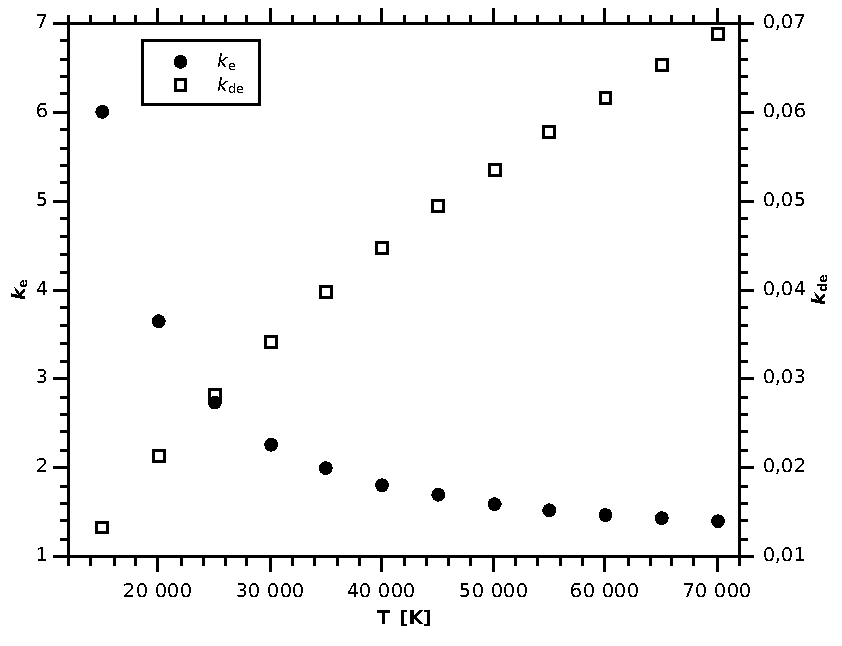
\includegraphics[width=13cm]{rk.pdf}
\caption{Závislost poměrů rychlostních koeficientů  $k_\mathrm{e}$ a~$k_\mathrm{de}$ na teplotě.}
\label{rk}
\end{center}
\end{figure}

\subsection{Experiment}

Na začátku byla provedena kontrola průtokoměrů. Byla měřena závislost tlaku v~reaktoru na průtoku. Průtokoměry fungovaly dobře, u manometrů se ukázalo, že jejich nulová hodnota se v~průběhu času mění, byla tedy naměřena nulová hodnota před a~po měření a~při výpočtech tlaků byla prováděna oprava o~tuto hodnotu. Závislosti tlaku v~reaktoru na průtoku kyslíku a~argonu jsou v~tabulkách \ref{prutokargon}, \ref{prutokkyslik} a~na obrázcích \ref{prutokar-img},\ref{prutoko2-img}. Výpočet $\eta$ a procentuální koncentrace argonu a kyslíku lze provést dvěma způsoby. Jednak přímo z průtoků a nebo, pokud si nejsme jistí správnou kalibrací průtokoměrů, můžeme neměřit závislost tlaku v reaktoru na průtoku a poměr následně vypočítat z parciálních tlaků. Vypočítané hodnoty jsou v tabulce \ref{prutokargon}.

\begin{table}[htbp]
\begin{center}
\begin{tabular}{|c|c|c|}
\hline
$Q_\mathrm{Ar}$ [sccm] & $p$ (Leybold) [Pa] & $p$ (MKS) [Pa] \\ \hline
0,139 & 0,24 & 0,2158 \\ \hline
0,278 & 0,51 & 0,4158 \\ \hline
0,417 & 0,72 & 0,5958 \\ \hline
0,556 & 0,87 & 0,7758 \\ \hline
0,695 & 1,07 & 0,9558 \\ \hline
0,834 & 1,13 & 1,1078 \\ \hline
0,973 & 1,28 & 1,268 \\ \hline
1,112 & 1,43 & 1,4194 \\ \hline
1,251 & 1,6 & 1,5652 \\ \hline
1,39 & 1,71 & 1,7102 \\ \hline
\end{tabular}
\caption{Závislost tlaku v~reaktoru na průtoku argonu.}
\label{prutokargon}
\end{center}
\end{table}

\begin{table}[htbp]
\begin{center}
\begin{tabular}{|c|c|c|}
\hline
$Q_\mathrm{O_2}$ [sccm] & $p$ (Leybold) [Pa] & $p$ (MKS) [Pa] \\ \hline
4,9 & 3,97 & 4,0522 \\ \hline
5,88 & 4,47 & 4,5764 \\ \hline
6,86 & 4,97 & 5,0728 \\ \hline
7,35 & 5,27 & 5,3191 \\ \hline
\end{tabular}
\caption{Závislost tlaku v~reaktoru na průtoku kyslíku.}
\label{prutokkyslik}
\end{center}
\end{table}

\begin{figure}[htbp]
\begin{center}
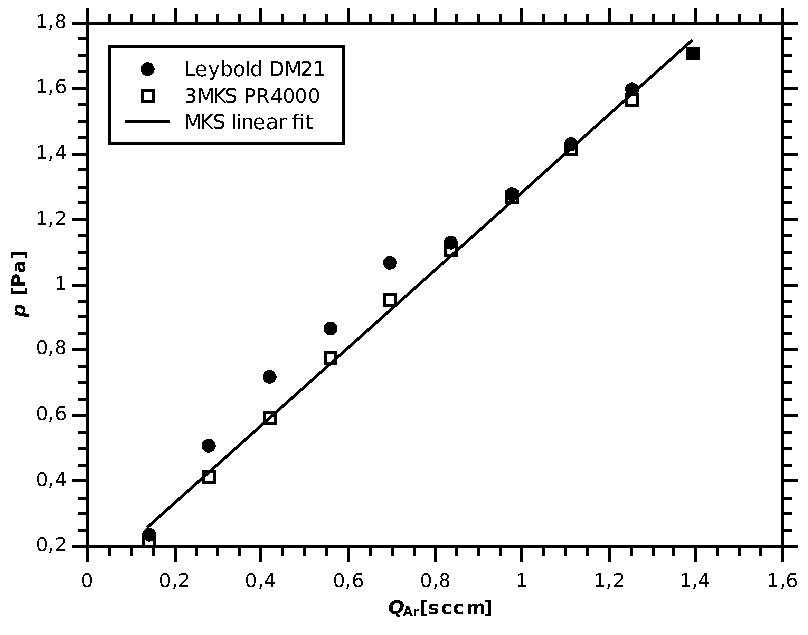
\includegraphics[width=12cm]{prutokar-img.pdf}
\caption{Závislost tlaku v~reaktoru na průtoku argonu.}
\label{prutokar-img}
\end{center}
\end{figure}

\begin{figure}[htbp]
\begin{center}
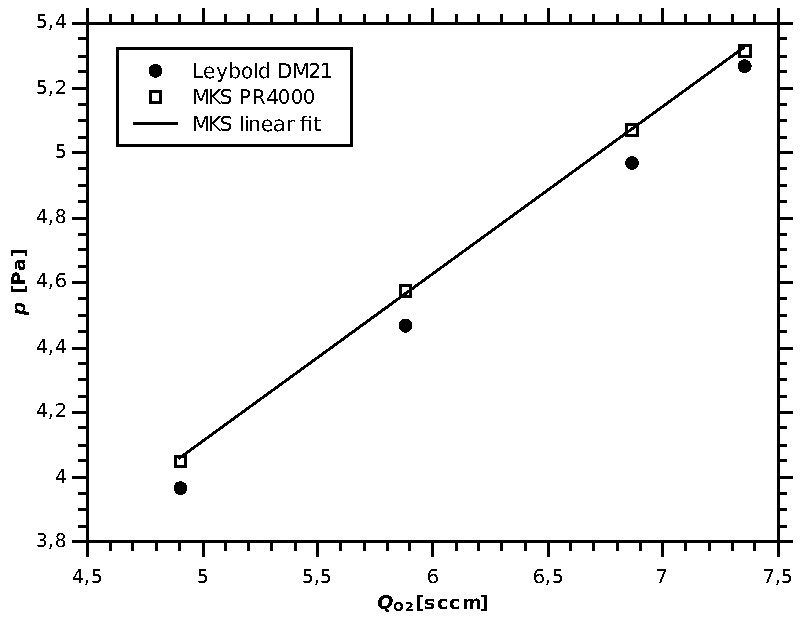
\includegraphics[width=12cm]{prutoko2-img.pdf}
\caption{Závislost tlaku v~reaktoru na průtoku kyslíku.}
\label{prutoko2-img}
\end{center}
\end{figure}



Na začátku měření byla provedena kontrola spektra, abychom se ujistili o~čistotě aparatury a~o~správné funkci spektrometru. Přítomnost žádné příměsi v~aparatuře se nepotvrdila, v~naměřených spektrech byly pozorovány pouze píky argonu a~kyslíku. I vlnové délky naměřených spektrálních čar dobře odpovídaly skutečnosti, po této stránce byl tedy spektrometr výborně funkční. 

Výrazně horší bylo rozlišení spektrometru a~šum. Na obrázku \ref{piky} je výřez spektra v~oblasti 730--860\,nm. Je vidět, že díky nízkému rozlišení spektrometru se blízké píky velmi slévají. Na obrázku \ref{tomas} je stejné spektrum, získané během stejného měření a~stejných podmínek druhou skupinou na spektrometru Triax (spektrum je převzato z~protokolu Tomáše Morávka). Spektra se od sebe velmi zásadně liší! Zatímco na obrázku ze spektrometru Triax můžeme zřetelně pozorovat jednotlivé píky a~šum je téměř nulový, na spektrometru Avaspec se píky bližší než 1--2\,nm slévají a~bohužel dochází v~tomto případě ke sčítání intenzit, což zásadním způsobem ovlivňuje celé měření, a~to proto, že oba píky používané při aktinometrii se nachází v~blízkosti jiných výrazných píků a~dochází k jejich ovlivnění. Pík kyslíku na 844,67\,nm je ještě víceméně v~pořádku, je zřetelně samostatný a~jeho intenzita pravděpodobně není moc ovlivněna blízkými píky argonu na 840,82 a~842,47\,nm. Naopak dva píky argonu na 750,38 a~751,46\,nm od sebe nelze nijak oddělit. Pro další měření byla tedy odečítána intenzita výsledného píku.

\begin{figure}[htbp]
\begin{center}
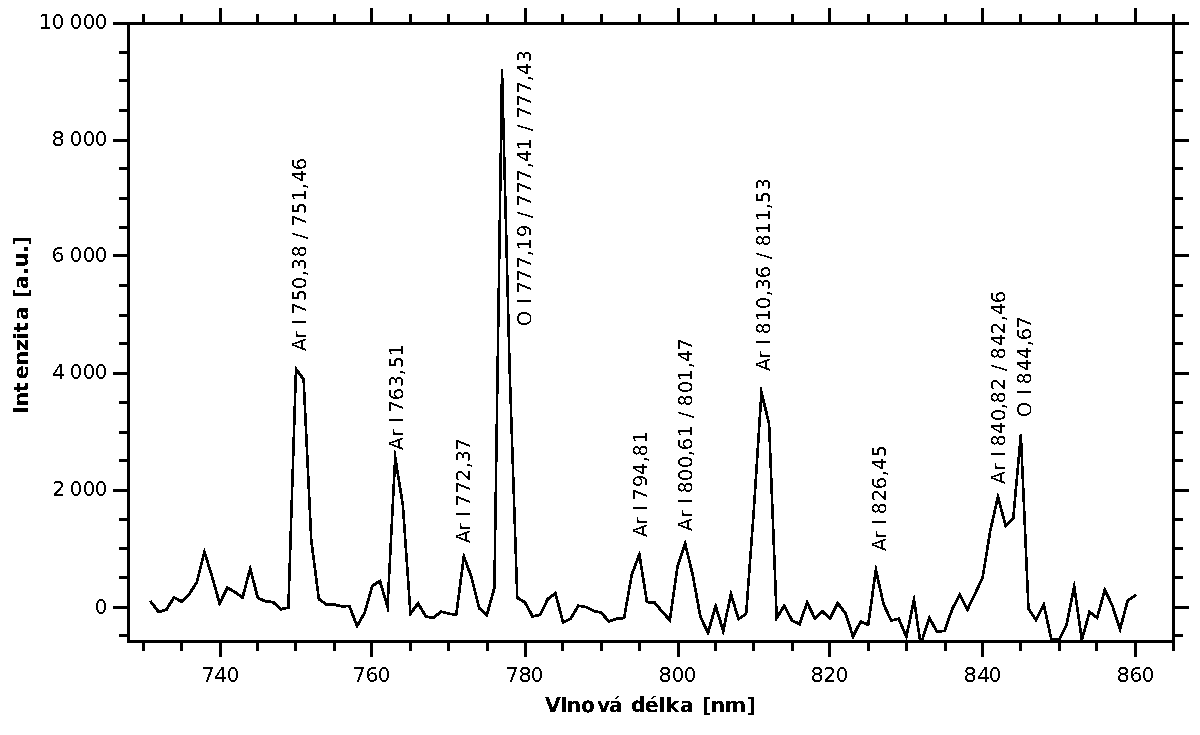
\includegraphics[width=21cm, angle=270]{piky.pdf}
\caption{Část naměřeného spektra s~identifikovanými píky.}
\label{piky}
\end{center}
\end{figure}

\begin{figure}[htbp]
\begin{center}
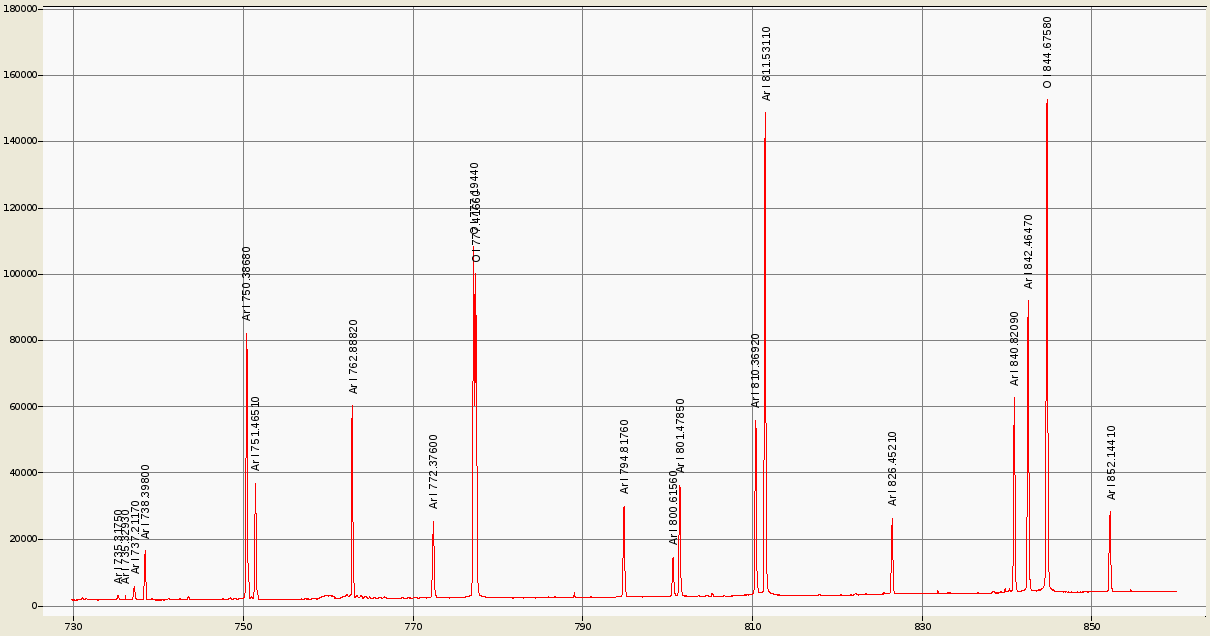
\includegraphics[width=21cm, angle=270]{triax.png}
\caption{Část naměřeného spektra na spektrometru Triax s~identifikovanými píky (převzato z~protokolu Tomáše Morávka).}
\label{tomas}
\end{center}
\end{figure}

Samotné měření bylo prováděno pro tři kombinace poměru koncentrací a tlaku:
\begin{itemize}
\item $p$ = 8,6\,Pa a $\eta$ = 7,05 (6,6\,\%Ar)
\item $p$ = 8,6\,Pa a $\eta$ = 14,1 (12,4\,\%Ar)
\item $p$ = 12,1\,Pa a $\eta$ = 14,1 (12,4\,\%Ar)
\end{itemize}
Pro každou konfiguraci byla měřena závislost stupně disociace a koncentrace radikálů na výkonu. Naměřené intenzity pro jednotlivé výkony a příslušné vypočítané stupně disociace a koncentrace kyslíkových radikálů jsou v tabulkách \ref{k1}, \ref{k2} a \ref{k3}. Byly také vypočítány poměry $\frac{1}{\eta C}\frac{I_{844}^\mathrm{O}}{I_{750}^\mathrm{Ar}}$ pro kontrolu podmínek (\ref{podm1}) a (\ref{podm2}). Závislosti stupně disociace a koncentrace kyslíkových radikálů na výkonu pro jednotlivé konfigurace jsou na obrázcích \ref{ioni} a \ref{conc}.

\begin{table}[htbp]
\begin{center}
\begin{tabular}{|c|c|c|c|c|c|}
\hline
$P$ [W] & $I_{750}^\mathrm{Ar}$ & $I_{844}^\mathrm{O}$ & $\frac{1}{\eta C}\frac{I_{844}^\mathrm{O}}{I_{750}^\mathrm{Ar}}$ & $\alpha_\mathrm{d}\,[\%]$ & [O]\,[$10^{19}$ m$^3$] \\ \hline
40 & 5884 & 640 & 0,098 & 1,48 & 5,34 \\ \hline
35 & 5656 & 671 & 0,107 & 1,71 & 6,14 \\ \hline
30 & 5452 & 632 & 0,105 & 1,65 & 5,92 \\ \hline
25 & 5203 & 575 & 0,100 & 1,52 & 5,48 \\ \hline
20 & 4834 & 522 & 0,098 & 1,47 & 5,27 \\ \hline
15 & 4368 & 444 & 0,092 & 1,32 & 4,75 \\ \hline
10 & 3758 & 362 & 0,087 & 1,20 & 4,32 \\ \hline
\end{tabular}
\caption{Data pro konfiguraci $p$ = 8,6\,Pa a $\eta$ = 7,05 (6,6\,\%Ar).}
\label{k1}
\end{center}
\end{table}

\begin{table}[htbp]
\begin{center}
\begin{tabular}{|c|c|c|c|c|c|}
\hline
$P$ [W] & $I_{750}^\mathrm{Ar}$ & $I_{844}^\mathrm{O}$ & $\frac{1}{\eta C}\frac{I_{844}^\mathrm{O}}{I_{750}^\mathrm{Ar}}$ & $\alpha_\mathrm{d}\,[\%]$ & [O]\,[$10^{19}$ m$^3$] \\ \hline
10 & 1896 & 380 & 0,091 & 1,29 & 4,94 \\ \hline
15 & 2243 & 504 & 0,102 & 1,57 & 6,00 \\ \hline
20 & 2440 & 588 & 0,109 & 1,75 & 6,71 \\ \hline
25 & 2598 & 647 & 0,113 & 1,84 & 7,06 \\ \hline
30 & 2746 & 722 & 0,119 & 2,00 & 7,67 \\ \hline
35 & 2874 & 792 & 0,125 & 2,14 & 8,22 \\ \hline
40 & 2958 & 855 & 0,131 & 2,30 & 8,81 \\ \hline
\end{tabular}
\end{center}
\caption{Data pro konfiguraci $p$ = 8,6\,Pa a $\eta$ = 14,1 (12,4\,\%Ar).}
\label{k2}
\end{table}


\begin{table}[htbp]
\begin{center}
\begin{tabular}{|c|c|c|c|c|c|}
\hline
$P$ [W] & $I_{750}^\mathrm{Ar}$ & $I_{844}^\mathrm{O}$ & $\frac{1}{\eta C}\frac{I_{844}^\mathrm{O}}{I_{750}^\mathrm{Ar}}$ & $\alpha_\mathrm{d}\,[\%]$ & [O]\,[$10^{19}$ m$^3$] \\ \hline
40 & 3279 & 889 & 0,123 & 2,09 & 12,6 \\ \hline
35 & 3134 & 838 & 0,121 & 2,05 & 12,3 \\ \hline
30 & 2997 & 758 & 0,114 & 1,89 & 11,3 \\ \hline
25 & 2818 & 680 & 0,109 & 1,75 & 10,5 \\ \hline
20 & 2594 & 602 & 0,105 & 1,65 & 9,89 \\ \hline
15 & 2311 & 505 & 0,099 & 1,49 & 8,97 \\ \hline
10 & 1933 & 385 & 0,090 & 1,27 & 7,64 \\ \hline
\end{tabular}
\end{center}
\caption{Data pro konfiguraci $p$ = 12,1\,Pa a $\eta$ = 14,1 (12,4\,\%Ar).}
\label{k3}
\end{table}



\begin{figure}[htbp]
\begin{center}
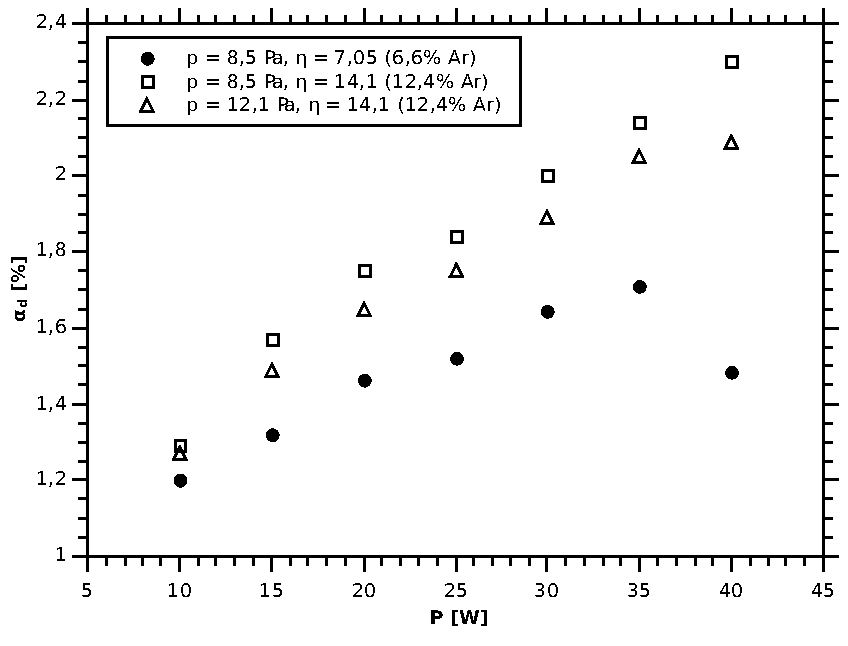
\includegraphics[width=12cm]{ionization.pdf}
\caption{Závislost stupně disociace na výkonu pro jednotlivé konfigurace.}
\label{ioni}
\end{center}
\end{figure}

\begin{figure}[htbp]
\begin{center}
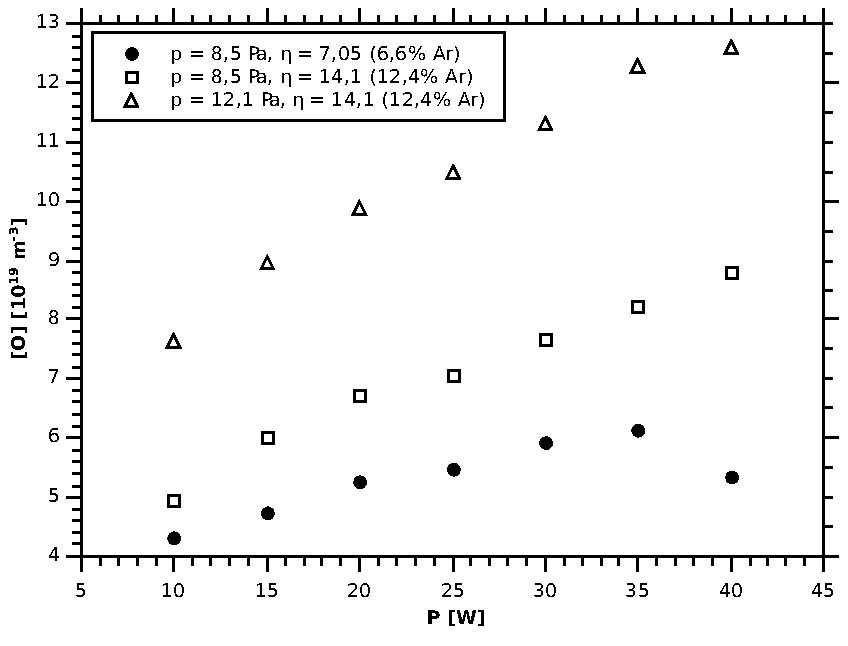
\includegraphics[width=12cm]{concentration.pdf}
\caption{Závislost koncentrace kyslíkových radikálů na výkonu pro jednotlivé konfigurace.}
\label{conc}
\end{center}
\end{figure}


\section{Závěr}
Měření proběhlo úspěšně. Podařilo se naměřit emisní spektra kyslíko-argonového plazmatu pro různé poměry argonu a kyslíku, pro různé tlaky a pro různé výkony. Z poměrů intenzit píků byly určeny stupně disociace a koncentrace kyslíkových radikálů. Pro všechna měření také byly splněny aktinometrické podmínky (\ref{podm1}) a (\ref{podm2}). Stupně disociace a koncentrace kyslíkových radikálů nicméně vyšly nižší než očekávané. To je dle našeho názoru způsobeno malým rozlišením spektrometru, což způsobilo, že do výsledné intenzity argonové čáry se připočítávala ještě čára vedlejší. Tím pádem vyšla intenzita $I_{750}^\mathrm{Ar}$ více, což se projevilo nižším než očekávaným stupněm disociace. Z tohoto důvodu si myslíme, že spektrometr Avaspec -- 2040TBC-2 je pro aktinometrické měření nevyhovující. Další problém je předpoklad, že se během měření teplota elektronů (a tedy i rychlostní koeficienty) nemění, což dle našeho názoru nebylo splněno. Další možnou chybou, které jsme se dopustili bylo použití Maxwellova rozdělení během výpočtu rychlostních koeficientů (toto se neshoduje s~výsledky získanými během sondových měření na stejném reaktoru v tomto praktiku). Z těchto důvodů byla odhadnuta chyba ve výsledcích na minimálně 100--200\,\%. 

\end{document}
